\documentclass{amsart}
\usepackage{amsmath, amssymb}

% For \includegraphics 
\usepackage{graphicx}

\title{Week 001}
\author{Kazuya Haine}
\date{}

\newcommand{\N}{\mathbb{N}}
\newcommand{\calC}{\mathcal{C}}

\newtheorem{theorem}{Theorem}

\newcounter{qpart}
\newcommand{\qpart}[1]{%
  \stepcounter{qpart}%
  \bigskip\noindent\textbf{(\alph{qpart})}\quad\textit{#1}\par\bigskip%
}

\begin{document}
\maketitle
Let $\calC$ be the collection of all finite subsets of $\N$, and let $\calC_n$ be the set of all subsets of $\N$ of $n$ elements, where $n \in \N$. 

\begin{theorem}[Schr\"oder-Bernstein]
    Suppose $f \colon A \to B$ and $g \colon B \to A$ are injections. Then there exists a bijection from $A$ to $B$.
\end{theorem}

\qpart{Show that $|\calC_k| = |\N^k|$ for all positive integers $k$.}

Consider the function $ord \colon \calC_k \to \N^k$ which takes an element $X \in \calC_k$ to the $k$-tuple consisting of the elements of $X$ in order. 
This is an injection since we can invert it: take the set containing each component of the $k$-tuple.

\bigskip
Consider the function $\N^k \to \calC_k$ given by the map
\[
    (n_1, n_2, \dots, n_k) \mapsto \{(r-1) + \sum_{i=1}^r n_i | r \in \{1, \dots, k\}\}.
\]
This function is an injection since we can invert it:
\begin{align*}
    \{(r-1) + \sum_{i=1}^r n_i | r \in \{1, \dots, k\}\} &\overset{ord}\mapsto (n_1, 1 + n_1 + n_2, \dots, k-1 + \sum_{i=1}^k n_i) \\
    &\overset{dif}\mapsto (n_1, n_2+1, \dots, n_k+1) \\
    &\overset{red}\mapsto (n_1, n_2, \dots, n_k)
\end{align*}
where the $dif$ map replaces the later terms with their difference to their previous term and $red$ reduces the result by subtracting 1 from every term except the first.

\medskip
Then $|\calC_k| = |\N^k|$ by applying Schr\"oder-Bernstein with these injections.

\qpart{Show, explicitly, that there is a bijection between $\N^2$ and $\N$.}

Consider the function $diag \colon \N^2 \to \N$ defined as follows:
\[
    (m,n) \mapsto m + \sum_{i=1}^{m+n} i.
\]
One can think of this function as ordering $\N^2$ primarily by the sum of components, with a fall back to the first component (see figure \ref{Cantor}).
\begin{figure}[h]
    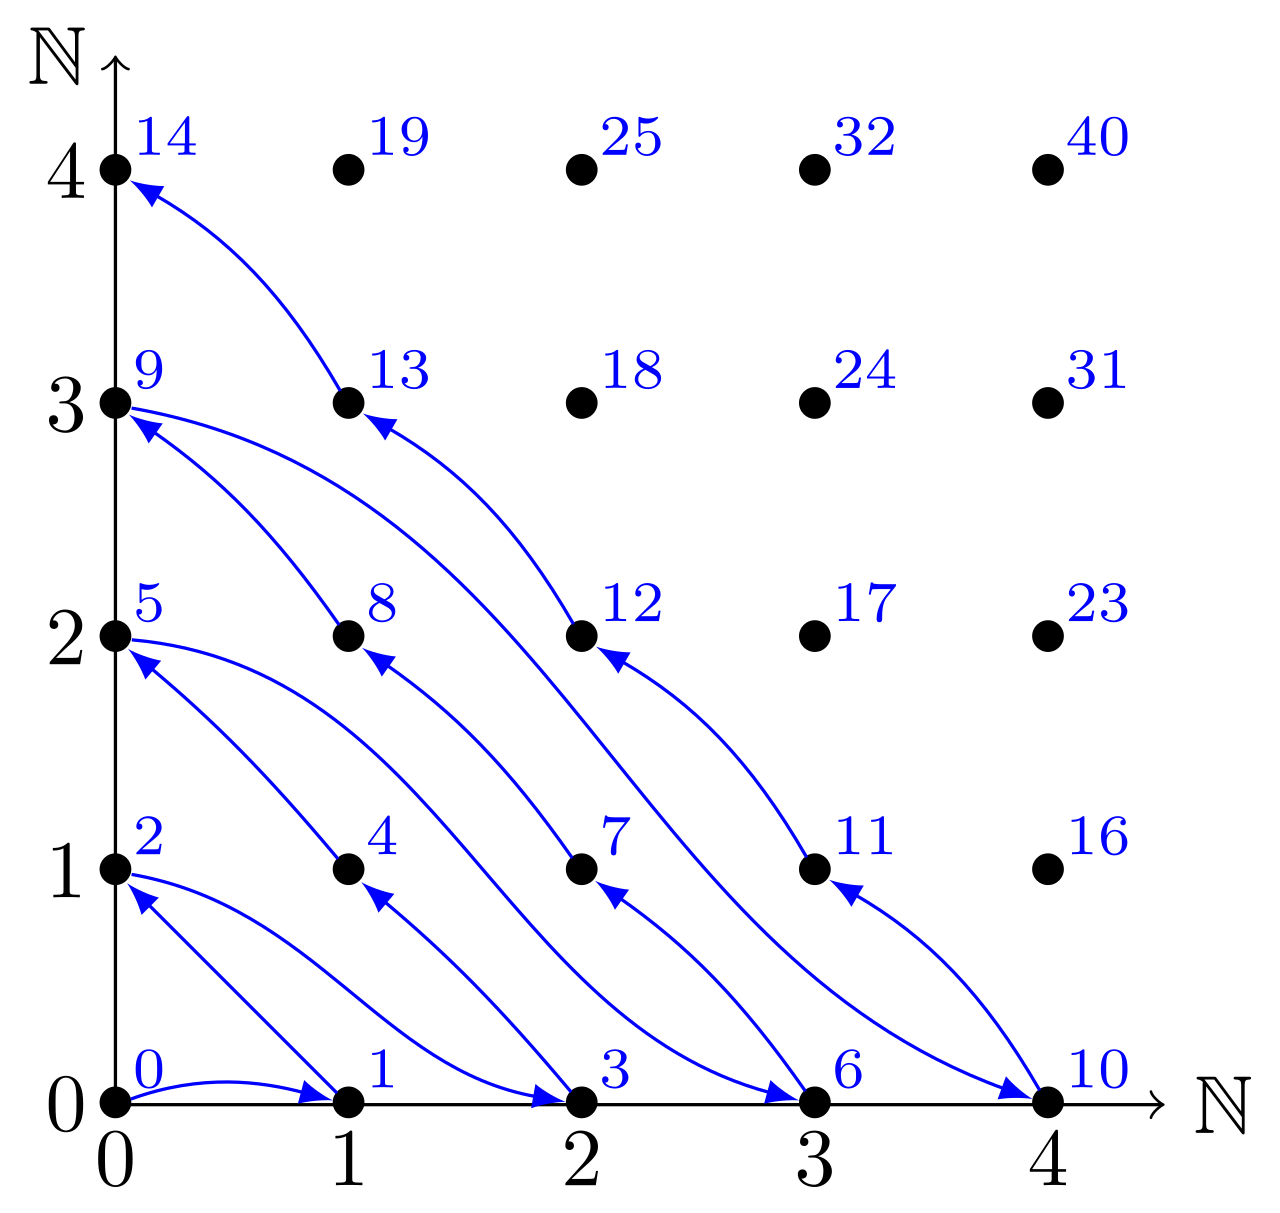
\includegraphics[width=0.5\textwidth]{Cantor_pairing.png}
    \caption{A diagram showing the ordering perspective.}
    \label{Cantor}
\end{figure}

\bigskip
As such, we can easily construct an inverse map $diag^{-1} \colon \N \to \N^2$. Indeed, to find $(m,n) := diag^{-1}(x)$ we first let $w$ be the index of the largest triangle number at most $x$.
Then let $t$ be the $w$th triangle number. Then we know that $m = x - t$ and $n = w - m$.
Putting these operations together forms a simple function which is easy to observe is the inverse of $diag$.

Unlike the previous inverses we've constructed, this acts on any element $n \in \N$, making it a total inverse rather than a partial inverse, and hence proving both functions are bijections, and thus that $|\N^2| = |\N|$.

\qpart{Show that $|\N^k| = |\N|$ for all positive integers $k$ by induction.}

To prove this by induction, we only need prove $|\N^{k+1}| = |\N|$ given that $|\N^k| = |\N|$ for each $k >= 2$ since it is trivial for $k = 1$.

\bigskip
Suppose that $|\N^k| = |\N|$, ie. we have a bijection $\N^k \overset{f_k}\longleftrightarrow \N$. Then we can compose bijections as follows, to obtain a bijection $\N^{k+1} \overset{f_{k+1}}\longleftrightarrow \N$:
\[
    \N^{k+1} = \N \times \N^k \overset{\operatorname{id}\times f_k}\longleftrightarrow \N \times \N = \N^2 \overset{diag}\longleftrightarrow \N.
\]

\qpart{By considering the fact that $\calC = \bigcup_{n\in\N}\calC_n$, show that $|\calC| = |\N|$.}

First, we observe that $|\calC_n| = |\N|$ for each natural $n$ (except 0) by composing the equalities from the previous parts. 
Thus, by observing that the union $\bigcup_{n\in\N}\calC_n$ is a disjoint union, we may immediately get 
\[
|\calC| = \left|\{\varnothing\}\sqcup\left(\bigsqcup_{n\in\N^+}\N\right)\right|.
\]
Formally, 
\[
    \bigsqcup_{n\in\N^+}\N := \{(n,x)\;|\;n\in\N^+,\;x\in\N\} = \N^+ \times \N
\]
Since $|\N^+| = |\N|$, $|\N^+ \times \N| = |\N^2| = |\N|$. So, $|\calC| = |\{\varnothing\}\sqcup \N|$. Thus, $|\calC| = |\N|$.

\begin{flushright}
Q.E.D.
\end{flushright}


\end{document}
